%% Copyright 2018 H.\ Rabus
%
% This work may be distributed and/or modified under the
% conditions of the LaTeX Project Public License, either version 1.3
% of this license or (at your option) any later version.
% The latest version of this license is in
%   http://www.latex-project.org/lppl.txt
% and version 1.3 or later is part of all distributions of LaTeX
% version 2005/12/01 or later.
%
% This work has the LPPL maintenance status `author-maintained'.
%
% This work consists of the file texbsp.tex
%

\documentclass[smallheadings]{scrartcl}

%%% GENERAL PACKAGES %%%%%%%%%%%%%%%%%%%%%%%%%%%%%%%%%%%%%%%%%%%%%%%%%%%%%%%%%%
% inputenc allows the usage of non-ascii characters in the LaTeX source code
\usepackage[utf8]{inputenc}
\usepackage{graphicx} 
%\graphicspath{ {/u/hnatiuka/Praktikum/PPI/} }



% title of the document
\title{Schnittstellendokumentation Serie 1\\Teil 1}
% optional subtitle
%\subtitle{Draft from~\today}
% information about the author
\author{%
  Arsen Hnatiuk,\\%
  Max Huneshagen 
}
\date{\today} 


%%% LANGUAGE %%%%%%%%%%%%%%%%%%%%%%%%%%%%%%%%%%%%%%%%%%%%%%%%%%%%%%%%%%%%%%%%%%
% babel provides hyphenation patterns and translations of keywords like 'table
% of contents'
\usepackage[ngerman]{babel}

%%% HYPERLINKS %%%%%%%%%%%%%%%%%%%%%%%%%%%%%%%%%%%%%%%%%%%%%%%%%%%%%%%%%%%%%%%%
% automatic generation of hyperlinks for references and URIs
\usepackage{hyperref}

%%% MATH %%%%%%%%%%%%%%%%%%%%%%%%%%%%%%%%%%%%%%%%%%%%%%%%%%%%%%%%%%%%%%%%%%%%%%
% amsmath provides commands for type-setting mathematical formulas
\usepackage{amsmath}
% amssymb provides additional symbols
\usepackage{amssymb}
% HINT
% Use http://detexify.kirelabs.org/classify.html to find unknown symbols!

%%% COLORS %%%%%%%%%%%%%%%%%%%%%%%%%%%%%%%%%%%%%%%%%%%%%%%%%%%%%%%%%%%%%%%%%%%%
% define own colors and use colored text
\usepackage[pdftex,svgnames,hyperref]{xcolor}

%%% Code Listings %%%%%%%%%%%%%%%%
% provides commands for including code (python, latex, ...)
\usepackage{listings}
\definecolor{keywords}{RGB}{255,0,90}
\definecolor{comments}{RGB}{0,0,113}
\definecolor{red}{RGB}{160,0,0}
\definecolor{green}{RGB}{0,150,0}
\lstset{language=Python, 
        basicstyle=\ttfamily\small, 
        keywordstyle=\color{keywords},
        commentstyle=\color{comments},
        stringstyle=\color{red},
        showstringspaces=false,
        identifierstyle=\color{green},
        }


\usepackage{paralist}
\usepackage{nicefrac}
% setting the font style for input und returns in description items
\newcommand{\initem}[2]{\item[\hspace{0.5em} {\normalfont\ttfamily{#1}} {\normalfont\itshape{(#2)}}]}
\newcommand{\outitem}[1]{\item[\hspace{0.5em} \normalfont\itshape{(#1)}]}
\newcommand{\bfpara}[1]{
	
	\noindent \textbf{#1:}\,}

\begin{document}

% generating the title page
\maketitle
% generating the table of contents (requires to run pdflatex twice!)
\tableofcontents
\bigskip

\hrule
\hrule

%%% BEGIN OF CONTENT %%%%%%%%%%%%%%%%%%%%%%%%%%%%%%%%%%%%%%%%%%%%%%%%%%%%%%%%%%

\section{Einleitung}

Aus der Theorie der Taylorentwicklung kann man ein günstiges Verfahren zur Approximation der ersten und zweiten Ableitungen einer Funktion ableiten: 
\begin{align}
\label{eq:1_abl}
f'(x)=\underbrace{\frac{f(x+h)-f(x)}{h}}_{:=D_h^{(1)}(x)}+\mathcal{O}(h)
\end{align}
bzw.
\begin{align}
\label{eq:2_abl}
f''(x)=\underbrace{\frac{f(x+h)-2f(x)+f(x-h)}{h^2}}_{:=D_h^{(2)}(x)}+\mathcal{O}(h^2)
\end{align}
mit der Differenziationsschrittweite $h$.

Die erstellten Skripte erlauben eine numerische Analyse dieses Verfahrens. Insbesondere wird der absolute Fehler dieses Verfahrens berechnet und sein Verlauf mit der Differenziationsschrittweite $h$ untersucht

\section{Schnittstellendokumentation \emph{differenzieren.py}}

Die in \emph{differenzieren.py} enthaltene Klasse \texttt{Differenzieren} erlaubt das Plotten von Funktionen und ihren Ableitungen. Die erste und zweite Ableitung kann dabei approximiert und mit der exakten Ableitung verglichen werden.

\subsection{Attribute}

\textbf{nicht-statische Attribute:}\\

\begin{compactdesc}
	\initem{ablex\_lis}{list}:~\\   Liste aus den ersten drei (anfangend bei 0) exakten Ableitungen der
            zu untersuchenden Funktion. Der list-Index gibt hierbei den Grad der
            Ableitung an, wobei die Funktion selbst als nullte Ableitung aufgefasst wird.
	      \initem{p\_arr}{numpy.ndarray aus floats}:~\\ Plotpunkte, an denen die Funktionen geplottet bzw. für die Fehlerbestimmung ausgewertet werden. Das Minimum dieses Arrays wird im Folgenden auch mit $a$ bezeichnet, das Maximum mit $b$.
\end{compactdesc}

\subsection{Konstruktor}

\texttt{Differenzieren(self, fkt, abl\_ex, abl2\_ex, p\_arr)}\\
Initialisiert ein neues Differenzieren-Objekt. Dazu müssen eine Funktion und die exakte erste und zweite Ableitung übergeben 
werden.

\bfpara{Input}
	    \begin{compactdesc}
		    \initem{fkt}{function}: ~\\ Bestimmt, wohin die Funktionen gezeichnet werden.
		    \initem{abl\_ex}{function}: ~\\ Exakte erste Ableitung.
		    \initem{abl2\_ex}{function}: ~\\ Exakte zweite Ableitung.
		   \initem{p\_arr}{numpy.ndarray aus floats}: ~\\ Plotpunkte, an denen die Funktionen geplottet bzw. für die Fehlerbestimmung
		                                                                                    aus gewertet werden.
	    \end{compactdesc}
\bfpara{Returns} -

\subsection{Methoden}
\subsubsection{plotfkt\_exakt}


\texttt{plotfkt\_exakt(self, plotbereich, grad=0, **kwargs)}\\
Plottet eine (\glqq exakte\grqq ) Funktion an den Plotpunkten in einen zu übergebenden Plot.
Man kann zwischen nullter, erster und zweiter Ableitung wählen.

\bfpara{Input}
	    \begin{compactdesc}
		    \initem{plotbereich}{pyplot.Axes-Objekt}: ~\\ Bestimmt, wohin die Funktion geplottet wird.
		    \initem{grad}{int, optional, Standard: 0}: ~\\ Grad der Ableitung. Bei grad==0 wird die Funktion selbst geplottet.
		    \initem{**kwargs}{keyword arguments, optional}: ~\\ Keyword arguments zur Übergabe an \texttt{pyplot.plot}. Nachzulesen in der
                \\ \texttt{matplotlib.lines.Line2D}-Doku.
	    \end{compactdesc}
\bfpara{Returns} -

\subsubsection{ablapprox}

\texttt{ablapprox(self, schrittw, grad=1)}\\
 Diese Funktion approximiert die erste oder zweite Ableitung der Funktion
        an den plotpunkten. Genutzt wird hierzu die Gleichung \eqref{eq:1_abl} bzw. \eqref{eq:2_abl}. Wird als Grad der zu approximierenden Ableitung 0
        angegeben, so wird der Funktionswert an der Plotpunkten zurückgegeben.
Zu beachten ist hierbei, das die Funktion auf dem Intervall $\left[a-h,b+h\right]$ definiert sein muss. Sollte dies nicht
der Fall sein, sollten als Plotpunkte entsprechend modifizierte Arrays gewählt werden. Da aber alle hier sinnvoll zu betrachtenden Funktionen auf ganz $\mathbb{R}$ definiert sein werden, stellt dies im Allgemeinen kaum eine praktische Einschränkung dar. 
Nennenswert ist außerdem, dass durch die durch \eqref{eq:1_abl} gegebene sog.~Vorwärtsmethode  für sehr große $h$
(i.~e. $h\gg\nicefrac{\vert a-b\vert}{p}$ mit der Anzahl der Plotpunkte $p$) zu einer \glqq Verschiebung\grqq der approximierten Ableitung und damit zu einer Vergrößerung des Fehlers führt. Dieses Artefakt ist allerdings in der doppelt-logarithmischen Darstellung der Fehler nicht sichtbar. Für kleine $h$ verliert dieser Effekt an Bedeutung, was diese Methode rechtfertigt, da die Konvergenz gegen $f'$ ja ohnehin erst für $h\rightarrow 0$ zu erwarten ist.


\bfpara{Input}
	    \begin{compactdesc}
		    \initem{schrittw}{float}: ~\\ Schrittweite der diskreten Differenziation.
		    \initem{grad}{int, optional, Standard: 1}: ~\\ Grad der gewünschten Ableitung. bei \texttt{grad==0} werden die Funktionswerte
                an den Plotpunkten zurückgegeben.
	    \end{compactdesc}
\bfpara{Returns}
       \begin{compactdesc}
		    \initem{~}{numpy.ndarray aus floats}: ~\\ Werte der gewünschten Ableitung der Funktion an den Plotpunkten.
	    \end{compactdesc}


\subsubsection{plotfkt\_approx}


\texttt{plotfkt\_approx(self, schrittw, plotbereich, grad=1, **kwargs)}\\
 Plottet die approximierte Ableitung (eines bestimmten Grades) der Funktion.
        Dabei wird die Funktion als nullte Ableitung aufgefasst.

\bfpara{Input}
	    \begin{compactdesc}
		    \initem{schrittw}{float}: ~\\ Schrittweite der diskreten Differenziation.
		    \initem{plotbereich}{pyplot.Axes-Objekt}: ~\\ Bestimmt, wohin die Funktion geplottet wird.
		    \initem{grad}{int, optional, Standard: 1}: ~\\ Grad der gewünschten Ableitung. bei \texttt{grad==0} wird die Funktion 
		                                                                                   selbst geplottet.
		    \initem{**kwargs}{keyword arguments, optional}: ~\\ Keyword arguments zur Übergabe an \texttt{pyplot.plot}. Nachzulesen in der
                \\ \texttt{matplotlib.lines.Line2D}-Doku.
	    \end{compactdesc}
\bfpara{Returns} -


\subsubsection{err\_abl}


\texttt{err\_abl(self, schrittw, grad=1)}\\
 Diese Funktion bestimmt das Maximum der absoluten Differenz zwischen approximierter
        Ableitung einer Funktion und der exakten Ableitung an den Plotpunkten.
        
\bfpara{Input}
	    \begin{compactdesc}
		    \initem{schrittw}{float}: ~\\ Schrittweite der diskreten Differenziation.
		    \initem{grad}{int, optional, Standard: 1}: ~\\ Grad der gewünschten Ableitung. bei \texttt{grad==0} wird als Fehler 0 zurückgegeben, da die Funktion selbst exakt gegeben ist.
		    \initem{**kwargs}{keyword arguments, optional}: ~\\ Keyword arguments zur Übergabe an \texttt{pyplot.plot}. Nachzulesen in der
                \\ \texttt{matplotlib.lines.Line2D}-Doku.
	    \end{compactdesc}
\bfpara{Returns}
       \begin{compactdesc}
		    \initem{~}{float}: ~\\ Maximale absolute Abweichung der approximierten Ableitung von \texttt{ablex}.
	    \end{compactdesc}

\subsection{Weitere Funktionen in \emph{differenzieren.py}}

\subsubsection{negsin}

\texttt{negsin(arg)}\\
 Da python-Funktionen nicht mit Skalaren multipliziert werden können, ist eine separate Definition des negativen Sinus,
 also der zweiten Ableitung des Sinus erforderlich.
        
\bfpara{Input}
	    \begin{compactdesc}
		    \initem{arg}{float}: ~\\ Stelle, die untersucht werden soll.
	    \end{compactdesc}
\bfpara{Returns}
       \begin{compactdesc}
		    \initem{~}{float}: ~\\ Wert von $-\sin$ an der Stelle \texttt{arg}.
	    \end{compactdesc}
	    
\subsubsection{test}

\texttt{test()}\\
Diese Funktion dient dem Testen der Klasse. Sie wird nur ausgeführt, wenn der Nutzer \glqq test\grqq als Kommando beim Ausführen von \emph{differenzieren.py} übergibt. Testweise wird für den Sinus eine Approximation der ersten beiden Ableitungen und der Vergleich mit den exakten Funktionen durchgeführt.
        
\bfpara{Input}-
\bfpara{Returns}-


%%%%%%%%%%%%%%%%%%%%%%%%%%%%%%%%%%%%%%%%%%%%%%%%%%%%%%%%%%%
%%%%%%%%%%%%%%%%%%%  Beginn Arsens Teil

\section{Bedienungsanleitung zum Hauptprogramm}

In der Datei \texttt{hauptprogramm.py} wird eine \texttt{main()} Methode implementiert. In dieser Methode werden alle Objekte erstellt, die später zur graphischen Darstellung des Fehlerplots dienen. Es werden auch die in der \texttt{differenzieren} Klasse definierten Methoden mittels der Beispielfunktion (Sinus) veranschaulicht. 

Zuerst wird der Benutzer aufgefordert, eine Schrittweite einzugeben. Es muss eine beliebige nichtnegative \texttt{float} Zahl eingegeben werden. Die Gültigkeit des Eingabetyps wird durch \texttt{exceptions} behandelt, und danach durch eine \texttt{if} Schleife auf Positivität geprüft. Eine nicht gültige Eingabe wird nicht berücksichtigt  und der Benutzer wird erneut gefordert, eine Eingabe zu machen.

Diese Kontrolle erfolgt auf die folgende Weise:

\begin{lstlisting}
abbr = 1 
while abbr == 1: 
    try:
        h_test = float(input('Mit welcher Schrittweite wollen Sie die' + 
        ' Ableitungen  approximieren?\n' +
        'Schreiben Sie bitte eine echt positive Zahl, z.B. 0.1\n'))
        abbr = 0
    except ValueError:
        print('Nicht gueltiger Wert eingegeben. Versuchen Sie erneut.')
        abbr = 1
    if h_test <= 0:
        print('Nicht gueltiger Wert eingegeben. Versuchen Sie erneut.')
        abbr = 1
\end{lstlisting}

Danach wird die Beispielfunktion (der Sinus) bearbeitet. Es werden Die \texttt{subplots} und die \texttt{arrays} erzeugt, auf welchen die Abbildungen geplottet und entsprechend evaluiert und approximiert werden. Ein Objekt der \texttt{differenzieren} Klasse für die Sinus Abbildung wird ebenfalls erzeugt.  Schließlich wird die Sinus Abbildung samt seiner  ersten beiden Ableitungen
und der Approximation (für die durch den Benutzer eingegebene Schrittweite) dieser Ableitungen mittels der in der \texttt{Differenzieren}-Klasse definierten Methoden graphisch dargestellt. Der absolute Fehler der Approximation jeder wird jeweils in der Standardausgabe angezeigt.

Anschließend wird die Funktion \texttt{fehlerplot()} aufgerufen, um die Beziehung zwischen dem absoluten Fehler und der Schrittweite zu veranschaulichen. 

\subsection{fehlerplot()}

In dieser Funktion wird ein Plot des absoluten Fehlers in Abhängigkeit von der Schrittweite mittels der Differenzieren Klasse gezeichnet. Diese Funktion benutzt insbesondere die \texttt{numpy.vectorize}-Methode, um Arrays mit den Fehlerwerten zu erzeugen, und die \texttt{numpy.loglog}-Methode, um eine doppelt-logarithmisch skalierte Graphik zu erstellen.

\bfpara{Input}
\begin{compactdesc}
	\initem{plotbereich}{pyplot.Axes-Objekt} Subplot, auf dem der Plot erzeugt wird
	\initem{diff\_objct}{Differenzieren-Instanz} Differenzieren-Objekt, das untersucht wird
	\initem{h\_array}{numpy.ndarray aus floats} Array mit den Schrittweiten
\end{compactdesc}

\bfpara{Returns}-


\subsection{Beispieldurchlauf}

Im Folgenden wird ein Beispieldurchlauf von \texttt{main()} demonstriert. Der eingegebene Wert für die Schrittweite ist 0.1.

\begin{verbatim}
Mit welcher Schrittweite wollen Sie die Ableitungen approximieren?
Schreiben Sie bitte eine echt positive Zahl, z.B. 0.1
0.1
Der absolute Fehler in der ersten Ableitung ist 0.04999, Schrittweite 0.1
Der absolute Fehler in der zweiten Ableitung ist 0.00083, Schrittweite 0.1
\end{verbatim}

Es werden dazu zwei Graphiken erzeugt (Abbildung \ref{Abbildung 1}). Man sieht auf der linken Seite eine Graphik mit dem absoluten Fehler als Funktion von der Schrittweite. Auf der rechten Graphik steht die Beispielfunktion mit ihren Ableitungen (exakt und approximiert). Man erkennt für diesen vergleichsweise großen $h$-Wert noch leicht die oben erwähnte \glqq Verschiebung\grqq der approximierten ersten Ableitung gegenüber der exakten Funktion. Der damit verbundene Fehler ist aber bereits hier hinnehmbar klein und lässt sich optisch schon ab $h=0.01$ nicht mehr wahrnehmen, während $h$ hier ohne Weiteres bis zu $h=10^{-10}$ verkleinert werden kann (s. Abbildung~\ref{Abbildung 1}).

\begin{figure}
	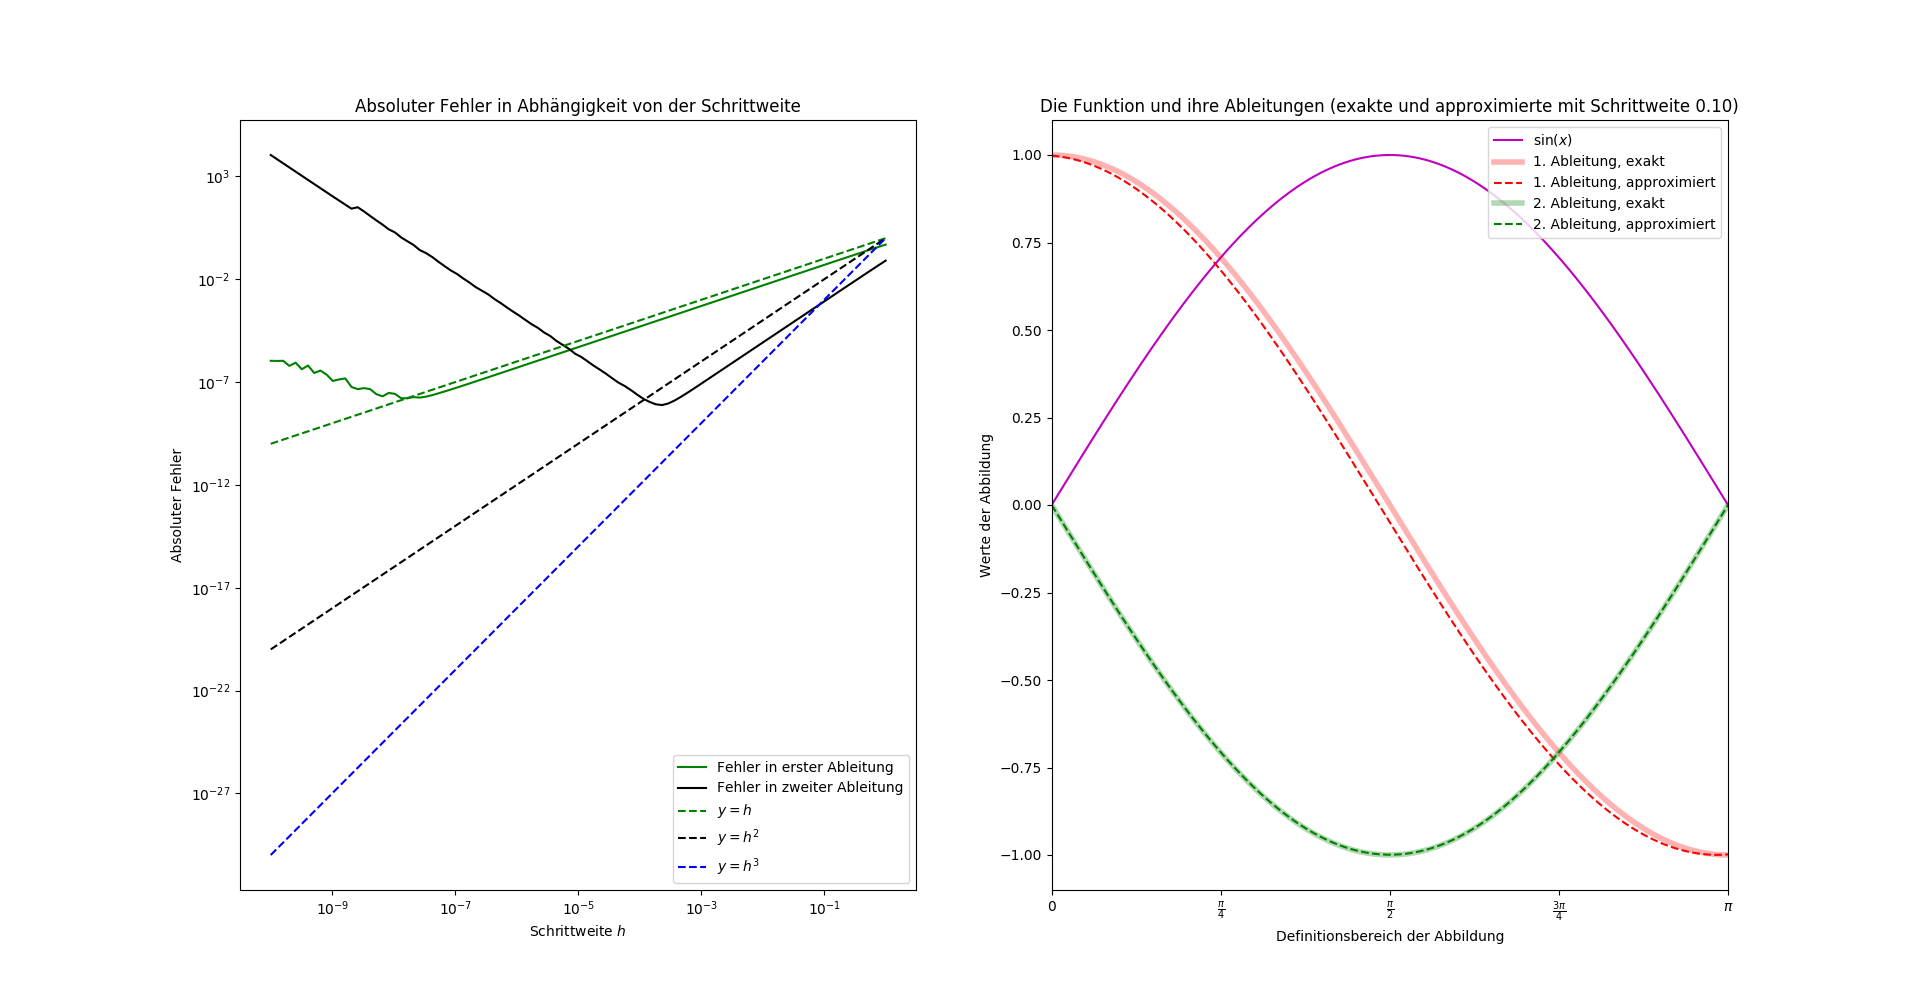
\includegraphics[width=\linewidth]{Figure_1.png}
	\caption{Die ausgegebene Graphik für $h=0.1$}
	\label{Abbildung 1}
\end{figure}

%%% END OF DOCUMENT %%%%%%%%%%%%%%%%%%%%%%%%%%%%%%%%%%%%%%%%%%%%%%%%%%%%%%%%%%%
\end{document}
